\section{Design Specification}

\subsection{Purpose}

The problem we are trying to solve is how to map a RESTful API onto a POSIX
filespace. This allows users to browse the data in a familiar topography and
also utilize various command-line tools for browsing, manipulating, creating,
and deleting data. 

Our program is meant to be used by an average user who has a basic understanding
of file systems and command-line tools. Our goal is to abstract the process so
that the user does not need to know the specific RESTful API, he or she simply
needs to know simple file operations in order to interact with the program.

\subsection{Overview}

For demonstration purposes we are basing our implementation off of the Twitter
API\footnote{http://http://dev.twitter.com/doc}. The Ruby middleware uses Sinatra
for pairing methods with RESTful routes. We use the ruby implementation of the
FUSE (Fileystem in User SpacE) \footnote{https://rubyforge.org/projects/fusefs/}
to actually mimic a POSIX filesystem on the user's local environment. All data
will be fetched from the API.

The FUSE driver maps a file system call to an HTTP verb. This HTTP request is
sent to a local instance of a web service

\begin{alltt}
	\$ ls vegasfs/users/ljsc/tweets.txt
\end{alltt} 

which is then processed by a sinatra handler:
	
\begin{alltt}
	get 'vegasfs/users/ljsc/tweets.txt' do
	  #handler
	end
\end{alltt}

This handler method will perform the actual call to the twitter service and
return the data as key:value pairs: 

\begin{alltt}
	Twitter::API.tweets\_for\_user(params[:user])
\end{alltt}

All internal messaging will be done by passing JSON objects containing key:value
pairs for twitter data and strings for URIs and verbs.

When redirected to a URL, the system should attempt to fetch the URL and save
locally. In the case of a common image file type (jpg,gif,png) the system should
attempt to recognize it and save as the appropriate file type. In the event of
another type of file, the system should create a reference link to be opened by
a web browser. These operations should be done utilizing CURL and other command
line tools as appropriate.  

\subsection{Top Level Archetecture}

\begin{figure}[h]
\centering
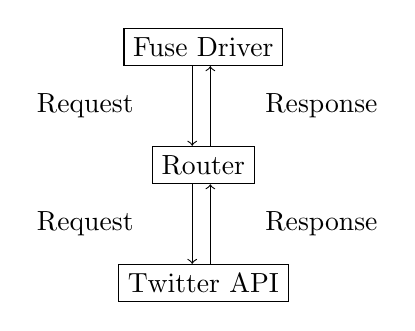
\begin{tikzpicture}
  \node [draw] at (0,3)    (Top)    {Fuse Driver};
  \node [draw] at (0,1.5)  (Middle) {Router};
  \node [draw] at (0,0)    (Bottom) {Twitter API};

  \draw [<-] (Bottom.120) -- (Middle.240);
  \draw [<-] (Middle.290) -- (Bottom.70);
  \draw [<-] (Middle.120) -- (Top.240);
  \draw [<-] (Top.290)    -- (Middle.70);

  \node at (-1.5, 0.75) { Request };
  \node at (-1.5, 2.25) { Request };
  \node at (1.5, 0.75)  { Response };
  \node at (1.5, 2.25)  { Response };
\end{tikzpicture}
\caption{Top Level Components}\label{fig:top-top}
\end{figure}

\subsubsection{Processing Elements}

\paragraph{The FUSE driver} handles file system requests generated due
to user actions on particular file paths as described in the requirements
document. It converts these requests into an HTTP request which is forwared to
the Sinatra backend.

\paragraph{The Router} implements a simple HTTP web server which listens to requests from
the FUSE driver. This will be implemented using the Sinatra framework, which
will match against a requested uri and invoke a specific handler. These handlers
will be responsible for fetching/manipulating the twitter data via the
webservice api provided by twitter.

\paragraph{Twitter API} will be leveraged to actually interact with the data as
requested by the user.  We will use an open source library for interacting with
twitter to get the required data.

\subsubsection{Connecting Elements and Data Elements}

The above processing elements are connected to form a layered architecture as
shown in figure~\ref{fig:top-top} above. All connections in the diagram
represent HTTP connections. An HTTP request using one of the specified verbs
(GET/POST/PUT/DELETE) is sent to lower level components from higher level
components. Likewise, lower level components will---based upon responses further
down the stack---return HTTP responses to the layer above.

